\documentclass[16pt, a4paper]{report}


\title{Gravitational Wave Astronomy}
\author{To be updated}
\date{\today}


\usepackage{amsmath}
\usepackage{tensor}
\usepackage{gensymb}
\usepackage[utf8]{inputenc}
\usepackage{graphicx}

\begin{document}
\maketitle

\pagebreak
Abstract here
\pagebreak

\pagebreak
\section{Introduction}
add general relativity work here
add spacetime work here
add history of gw work here
add explanation of gw here
\pagebreak

\pagebreak

\section{Linearized theory of Gravitational waves}

Einstein's field equations 
\begin{equation}
    G_{\mu\nu}= \frac{8 \pi  G}{c^{4}}  T_{\mu\nu}
\end{equation}
is a tensor equation which describes gravity in form of Einstein's tensor, $G_{\mu\nu}$ which is directly dependent on the geometry of space-time which is altered by the stress-energy tensor $T_{\mu\nu}$

Another field equation that relates the geometry or curvature of space-time to stress-energy tensor is 

\begin{equation}
    R_{\mu\nu}-\frac{1}{2}g_{\mu\nu}R=\frac{8\pi G}{c^{4}}T_{\mu\nu}
\end{equation}
where $R_{\mu\nu}$ is the Riemann tensor which describes the curvature of space-time, $R$ is the scalar curvature and $g_{\mu\nu}$ is the gravitational field tensor.

Any change in matter distribution will be recorded in in $T_{\mu\nu}$. So if $T_{\mu\nu}$ changes then according to equation 2, gravitational field tensor $g_{\mu\nu}$ also has to change. 

If $h_{\mu\nu}$ is the variation induced in space-time then the new gravitational field tensor $\tilde{g}_{\mu\nu}$ is given by 

\begin{equation}
    \tilde{g}_{\mu\nu} = g_{\mu\nu} + h_{\mu\nu}
\end{equation}

To get the new gravitational field, Einstein's field equation should be solved for $\tilde{g}_{\mu\nu}$ which gives 

\begin{equation}
    \tilde{h}_{\mu\nu} = h_{\mu\nu} - \frac{1}{2} \, \eta_{\mu\nu} \, h^{\alpha}_{\alpha}
\end{equation}
 where $\eta_{\mu\nu}$ is the gravity where space is flat i.e. $\eta_{\mu\nu} = g_{\mu\nu}$ and $h^{\alpha}_{\alpha}$ is summed for all spatial coordinates i.e. $\alpha$ takes values $(1,2,3) $ which corresponds to $(x,y,z)$.
 
 The admitted solutions for this variations in space time $\tilde{h}_{\mu\nu}$ has solution in the form of 
 
 \begin{equation}
     \tilde{h}_{\mu\nu} = A^{\mu\nu}\, e^{ik_{\alpha}x^{\alpha}}
 \end{equation}
 
 which is a 3D wave equation where $A^{\mu\nu}$ is the Amplitude tensor, $i = \sqrt{-1} $, $k_{\alpha} = (k_{x},k_{y},k_{z})$ is the wave vector and $x^{\alpha} = (x^{1},x^{2},x^{2}) = (x,y,z)$ is the position vector.
\pagebreak

\section{Properties of Gravitational waves}
\subsection{Polarization of Gravitational waves}
The amplitude tensor $A^{\mu\nu}$ has two forms $A^{\mu\nu}_{+}$ and $A^{\mu\nu}_{\times}$ which are orthogonal to each other. They can be represented as 

\begin{equation}
    A^{\mu\nu}_{+} = h_{+}\, \varepsilon^{\mu\nu}_{+}
\end{equation}

\begin{equation}
    A^{\mu\nu}_{\times} = h_{\times} \,\varepsilon^{\mu\nu}_{\times}
\end{equation}

where $\varepsilon^{\mu\nu}_{+}$ and $\varepsilon^{\mu\nu}_{\times}$ are unit polarization tensors.

\begin{equation}
\varepsilon^{\mu\nu}_{+} =
\begin{bmatrix}
0 & 0 & 0 & 0 \\
0 & +1 & 0 & 0 \\
0 & 0 & -1 & 0 \\
0 & 0 & 0 & 0 \\
\end{bmatrix}
\end{equation}
\\
\begin{equation}
\varepsilon^{\mu\nu}_{\times} =
\begin{bmatrix}
0 & 0 & 0 & 0 \\
0 & 0 & +1 & 0 \\
0 & +1 & 0 & 0 \\
0 & 0 & 0 & 0 \\
\end{bmatrix}
\end{equation}

\noindent In general relativity any tensor with indices $\mu\nu$ is a rank 2 tensor with 4 rows and 4 columns where each index can take values of space time coordinates which are $(t,x,y,z)$ , and position of each element is associated with any two coordinates. Thus in such tensors, the positions of elements are associated with space-time as follows:

\begin{equation*}
    \begin{bmatrix}
    tt & tx & ty & tz \\
    xt & xx & xy & xz \\
    yt & yx & yy & yz \\
    zt & zx & zy & zz \\
    \end{bmatrix}
\end{equation*}

So when we compare the unit polarization tensors $\varepsilon^{\mu\nu}_{+}$ and $\varepsilon^{\mu\nu}_{\times}$ with the above one, we see that in $\varepsilon^{\mu\nu}_{+}$ the non zero entries are +1 in $`xx$' direction and -1 in $`yy$' direction, hence the $A^{\mu\nu}_{+}$ amplitude is oriented only along X and Y axes, thus this gravitational wave which oscillates along X and Y axes is called as `PLUS' polarized wave because the vibration resembles `+' symbol. But in $\varepsilon^{\mu\nu}_{\times}$ the non zero entries are +1 in $`xy$' direction and -1 in $`yx$' direction, hence the $A^{\mu\nu}_{+}$ amplitude is oriented in the `XY' plane at a an angle of 45$\degree$ to the axes, thus this gravitational wave which oscillates in the `XY' plane at a an angle of 45$\degree$ to the axes is called as `CROSS' polarized wave because the vibration resembles `$\times$' symbol. 
\\

So the equation of polarized gravitational waves are:-\\
(+) wave $\Rightarrow $  $\tilde{h}_{\mu\nu} = h_{+}\, \varepsilon^{\mu\nu}_{+}\, e^{i(\omega t - k_{z}z)}$\\
$(\times)$ wave $\Rightarrow $  $\tilde{h}_{\mu\nu} = h_{\times}\, \varepsilon^{\mu\nu}_{\times}\, e^{i(\omega t - k_{z}z)}$

\subsection{Effect of Gravitational waves on objects}
\subsubsection{Plus polarized effect}
When a plus polarized wave passes through the object, since such gravitational wave makes space-time oscillate in X and Y axes only. So the points in space along axis will come close during compression and go far during stretching. Thus the object itself will be compressed and stretched along the axes, perpendicular to the direction of propagation of wave.

\subsubsection{Cross polarized effect}
When a cross polarized wave passes through the object, since such gravitational wave makes space-time oscillate along the line which makes an inclination of 45$\degree$ with X and Y axes (i.e. along the line $x=y$ and $x=-y$). So the points in space along those line will come close during compression and go far during stretching. Thus the object itself will be compressed and stretched along those lines, perpendicular to the direction of propagation of wave.
\\

Thus for every phase difference of $\pi/2$ we get the shape of object to be as follows
when a plus polarized wave passes and a cross polarized wave passes through a spherical object:

\begin{center}
    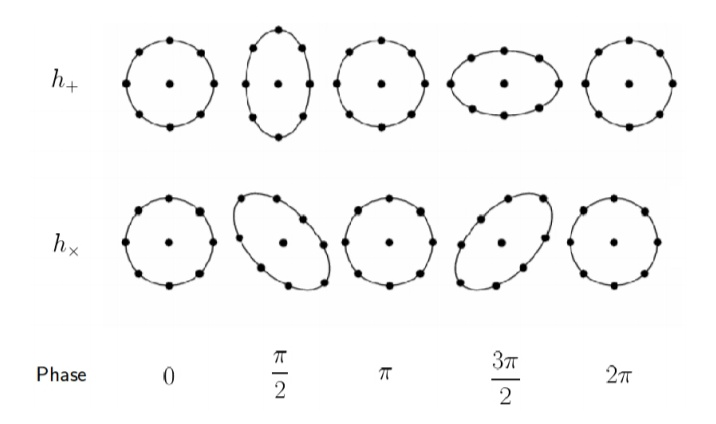
\includegraphics[scale=0.5]{images.tex/effect_of_gw.jpeg}
\end{center}


%add your work in form of folders and use \input{folder_name.tex/file_name}

\end{document}
